\documentclass[]{elsarticle} %review=doublespace preprint=single 5p=2 column
%%% Begin My package additions %%%%%%%%%%%%%%%%%%%
\usepackage[hyphens]{url}



\usepackage{lineno} % add
\providecommand{\tightlist}{%
  \setlength{\itemsep}{0pt}\setlength{\parskip}{0pt}}

\bibliographystyle{elsarticle-harv}
\biboptions{sort&compress} % For natbib
\usepackage{graphicx}
\usepackage{booktabs} % book-quality tables
%%%%%%%%%%%%%%%% end my additions to header

\usepackage[T1]{fontenc}
\usepackage{lmodern}
\usepackage{amssymb,amsmath}
\usepackage{ifxetex,ifluatex}
\usepackage{fixltx2e} % provides \textsubscript
% use upquote if available, for straight quotes in verbatim environments
\IfFileExists{upquote.sty}{\usepackage{upquote}}{}
\ifnum 0\ifxetex 1\fi\ifluatex 1\fi=0 % if pdftex
  \usepackage[utf8]{inputenc}
\else % if luatex or xelatex
  \usepackage{fontspec}
  \ifxetex
    \usepackage{xltxtra,xunicode}
  \fi
  \defaultfontfeatures{Mapping=tex-text,Scale=MatchLowercase}
  \newcommand{\euro}{€}
\fi
% use microtype if available
\IfFileExists{microtype.sty}{\usepackage{microtype}}{}
\usepackage{graphicx}
% We will generate all images so they have a width \maxwidth. This means
% that they will get their normal width if they fit onto the page, but
% are scaled down if they would overflow the margins.
\makeatletter
\def\maxwidth{\ifdim\Gin@nat@width>\linewidth\linewidth
\else\Gin@nat@width\fi}
\makeatother
\let\Oldincludegraphics\includegraphics
\renewcommand{\includegraphics}[1]{\Oldincludegraphics[width=\maxwidth]{#1}}
\ifxetex
  \usepackage[setpagesize=false, % page size defined by xetex
              unicode=false, % unicode breaks when used with xetex
              xetex]{hyperref}
\else
  \usepackage[unicode=true]{hyperref}
\fi
\hypersetup{breaklinks=true,
            bookmarks=true,
            pdfauthor={},
            pdftitle={Time Preferences in Job Search From South Africa to China},
            colorlinks=false,
            urlcolor=blue,
            linkcolor=magenta,
            pdfborder={0 0 0}}
\urlstyle{same}  % don't use monospace font for urls

\setcounter{secnumdepth}{0}
% Pandoc toggle for numbering sections (defaults to be off)
\setcounter{secnumdepth}{0}
% Pandoc header
\usepackage{float}



\begin{document}
\begin{frontmatter}

  \title{Time Preferences in Job Search From South Africa to China}
    \author[Smith College]{Zoya Azhar\corref{c1}}
   \ead{zazhar@smith.edu} 
   \cortext[c1]{Corresponding Author}
    \author[Smith College]{Emeline Cox}
   \ead{ecox@smith.edu} 
  
    \author[Smith College]{Yejin Hwang}
   \ead{yhwang67@smith.edu} 
  
    \author[Smith College]{Kelly Pien}
   \ead{kpien@smith.edu} 
  
      \address[Smith College]{Department of Economics, Pierce Hall, Northapmton, MA, 01063}
  
  \begin{abstract}
  Job-seeking is a key part of individual economic decision making. Often,
  however, people do not use optimal search strategies in job search. They
  intend to search for longer than they do, and do not make concrete plans
  that are easy to follow, leading to differences in preferences and
  behaviors across time. This paper examines the ``intention-behavior
  gap,'' an idea that Abel et al. (2019) talks about in the context of
  unemployed youth in South Africa, and discusses existing literature. It
  specifically focuses on the effects of different interventions,
  including workshops, plan-making, and career counseling, and questions
  whether the gap can be bridged by affecting behaviors. \par
  \textbf{JEL Classification:} D90 \par
  \textbf{Keywords:} Behavioral, Microeconomics, Present Bias, Time
  Inconsistency
  \end{abstract}
  
 \end{frontmatter}

\section{1. Introduction}\label{introduction}

Behavioral economics (BE) uses insights from decision psychology,
behavioral game theory, neuroeconomics, and related fields to understand
the real-world preferences and choices of economic actors. Time
preferences are particularly useful to examine through a BE lens, as
most people exhibit preferences over time that are not classically
rational (not transitive and consistent over time) and may make
immediate choices that do not maximize long-term expected utility, or
that lead to predictable regrets. One important application of temporal
decision-making is in job search. Our main paper, by Abel et al. (2019),
notes significant differences between what individuals state they intend
to do when searching for jobs and their actual behaviors. The paper
focuses on young job seekers in South Africa. It reports that many job
seekers search for jobs for fewer hours than they intend. It also found
that some planning techniques significantly increased the number of
applications submitted and the likelihood that job seekers would hear
back from employers, although the number of hours spent searching didn't
increase.

Our project furthers Abel et al.'s study by examining the observed
intention-behavior gap more closely. Our research question is as
follows: What causes the ``intention-behavior gap'', and can it be
bridged most effectively by altering planning and behaviors via
well-defined interventions? We framed this question in terms of trying
to carefully observe indicators (stated intentions of goals or
subsequent behaviors in executing them) of the underlying cause(s) of
the ``intention-behavior gap'' in order to find the most effective way
to bridge it to help job seekers to make more efficient use of their
search time.We explore whether intentions or behaviors are more in need
of change: do unreasonable expectations fall apart in practice, or does
procrastination ruin good intentions (or both)? Our design for testing
this question involves a time-series analysis involving looking at
job-seekers both before and after our interventions. Specifically, we
examine the effects of the following treatments: (a) informational
workshops (which affect preparatory job search and change individuals'
job-seeking strategies), (b) workshops that provided employer-specific
information (c) career counseling with a professional job-counselor
(peer counseling was not found to be particularly useful by Abel et al.,
but other research suggests that professional counseling may help,
particularly as found in a paper by Hoven et al. (2016) discussed in our
literature review), (d) action-plan creation (which Abel et al.
suggested might be most effective for combating procrastination effects
brought about by the cognitive load of tackling complex and unfamiliar
tasks), and (e) a control group.

We propose to focus on job-seekers in China in order to not only focus
on a different market but also to test the extent that
employment-specific information affects job-search. Some literature
relevant to our new design was specific to job-search, but in different
countries such as Germany. Others had different contexts such as
students and procrastination in college, but overall, each grappled with
time-inconsistent behavior.

\section{2. Summary and Reproduction of Abel et al.
(2019)}\label{summary-and-reproduction-of-abel_bridging_2019}

\subsubsection{Main Conclusions}\label{main-conclusions}

\emph{Bridging the Intention Gap? The Effect of Plan-Making Prompts on
Job Search and Employment} by Abel et al. (2019) argues that there is an
``intention gap'' between good intentions and actual behaviors of young
job seekers in South Africa: they intend to undertake certain behaviors
for seeking jobs, but end up behaving differently in practice, due in
large part to psychological and behavioral biases that create dynamic
inconsistencies between plans and behaviors over time. The paper tries
to ``bridge'' the gap by applying different treatments to change
behaviors. The focus is on ``Plan-Making Prompts,'' or helping
job-seekers to form plans that will lead to more efficient job-search
behavior (i.e.~dropping off more CVs, increasing the number of job
applications, etc.) By increasing the efficiency of job search and
increasing the number of job applications submitted, the intervention
helps to make job search easier and more likely to lead to employment.

\subsubsection{Methods}\label{methods}

The experimental interventions that Abel et al. conducted focused on job
seekers in South Africa between the ages of 18 and 35 who had registered
with the Employment Services of South Africa and who were able to travel
to the Labor Centers where the study was conducted. The sample included
1,097 unemployed youths who were actively seeking work and who spent
roughly 11 hours per week on job search but who submitted very few
applications (roughly 4.4 in a month). The study randomly assigned
participants to one of three main treatments: a control group (Control),
a group that attended a workshop (Workshop), and a group that attended a
workshop and completed an action plan (WorkshopPlus). The workshops were
run by career counselors and covered topics that included job search
strategies, CV creation, and interview techniques. They provided
information about resources for job search. The action plan group also
filled out a chart that encouraged them to think about their schedules
and formulate specific, concrete goals for job search and specific tasks
they could complete, such as setting a certain number of hours for job
search or a number of applications they were planning to submit.

Additionally, there were two sub-treatments. Within the WorkshopPlus
group, some individuals were randomly asked to nominate a peer to help
them with their search. In the Workshop and WorkshopPlus groups, some
participants were randomly assigned to receive text message reminders,
either about topics covered in the workshop for the former or about the
goals listed in the action plan for the latter.

Finally, the main paper supplemented the survey data with an observed
measure of job search by sending participants a ``text message (from a
number they could not associate with the research study)'' that notified
them of an actual vacancy in a specific sector (whenever possible in a
sector in which they worked before) (Abel et al. (2019)). It invited
them to submit an application to a specific email address which allowed
the researchers to observe whether the participants responded to the
message and to evaluate the quality of the material submitted.

\subsubsection{Results and Conclusions}\label{results-and-conclusions}

The first conclusion the paper drew was that the number of hours spent
searching for jobs did not increase in either of the two main
intervention groups. In the group that completed the action plan,
however, the number of applications significantly increased when
compared to the control and to the group that just attended the
workshop. Additionally, job-seekers in the action plan group tended to
receive more responses from employers. Abel et al. concluded that this
was not due to significantly better applications than those found in the
workshop group. Instead, they found that people in the action plan group
tended to diversify their search strategies and tried more
non-application based strategies, such as dropping off more CVs or
answering more job advertisements. This may have been because less-used
job search channels tend to be higher effort, and the job-seekers in the
action plan group were able to break down high-effort tasks into more
manageable sub-tasks. In short, action plans help bridge the
``intention-behavior gap'' by translating good intentions into easily
completed tasks which leads to more effective job-search behavior.

\subsubsection{Reproduction}\label{reproduction}

This section of our paper will discuss the reproduction of relevant
figures and regression results presented in Abel et al. (2019). The
regression tables and figures are in included in this section. We were
mostly successful, except we were not able to reproduce the line in the
regression tables with the control means.

\begin{table}[H] \centering 
  \caption{Sample Characteristics} 
  \label{} 
\begin{tabular}{@{\extracolsep{5pt}}lcccc} 
\\[-1.8ex]\hline 
\hline \\[-1.8ex] 
Statistic & \multicolumn{1}{c}{N} & \multicolumn{1}{c}{Mean} & \multicolumn{1}{c}{Median} & \multicolumn{1}{c}{St. Dev.} \\ 
\hline \\[-1.8ex] 
Age & 1,097 & 26.686 & 26.000 & 4.467 \\ 
Female & 1,097 & 0.518 & 1.000 & 0.500 \\ 
Years.of.schooling & 1,096 & 12.123 & 12.000 & 1.159 \\ 
Household.size & 1,097 & 2.363 & 2.000 & 1.910 \\ 
Moved.to.Johannesburg & 1,097 & 0.298 & 0.000 & 0.458 \\ 
Ever.employed & 1,097 & 0.794 & 1.000 & 0.405 \\ 
Reservation.wage & 1,091 & 3,162.126 & 3,000.000 & 1,832.972 \\ 
Fair.wage & 1,097 & 5,800.365 & 5,000.000 & 3,209.012 \\ 
Job.search.transport.cost & 1,043 & 76.919 & 45.000 & 91.728 \\ 
Number.employed.friends & 1,097 & 1.876 & 1.000 & 2.081 \\ 
Job.search.hours..week. & 1,058 & 11.353 & 8.000 & 9.874 \\ 
Job.applications..month. & 1,087 & 4.362 & 3.000 & 5.257 \\ 
\hline \\[-1.8ex] 
\end{tabular} 
\end{table}

Note: This table reports summary statistics at the baseline and is
winsorized at the ninety-fifth percentile.

\begin{table}[H] \centering 
  \caption{Action-Plan Descriptives} 
  \label{} 
\begin{tabular}{@{\extracolsep{5pt}}lccc} 
\\[-1.8ex]\hline 
\hline \\[-1.8ex] 
Statistic & \multicolumn{1}{c}{N} & \multicolumn{1}{c}{Mean} & \multicolumn{1}{c}{St. Dev.} \\ 
\hline \\[-1.8ex] 
Goal..Opportunities.to.identify & 339 & 10.348 & 6.497 \\ 
Goal..Applications.to.submit & 340 & 7.821 & 4.332 \\ 
Goal..Job.search.hours & 345 & 8.458 & 5.783 \\ 
Activity.days & 357 & 3.751 & 2.377 \\ 
Completed.AP & 402 & 0.888 & 0.316 \\ 
\hline \\[-1.8ex] 
\end{tabular} 
\end{table}

Notes: This table shows the characteristics of transcribed action plans.
Activity days refer to the number of days on which an activity was
listed. Respondents listed goal hours, opportunities, and applications
following the weekly breakdown of activities.

Our reproduction of Tables 1 and 2 contain exactly the same content as
the paper's. Tables 1 and 2 show summary statistics for the study
participants and their job search plans, respectively.

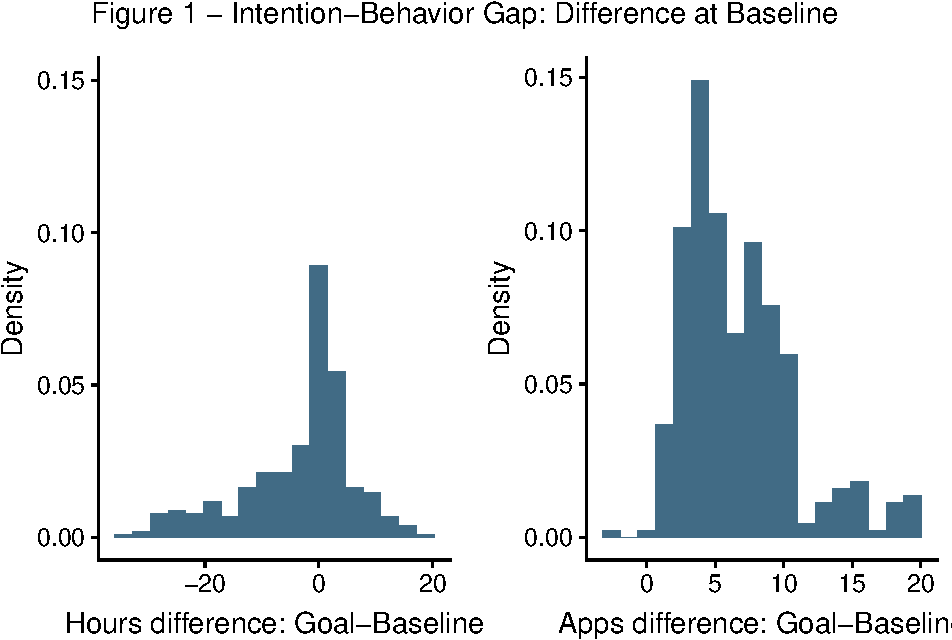
\includegraphics{project_template_files/figure-latex/figure1-1.pdf}
Note: This figure shows the distribution of the difference between
search intentions (search hours and submitted applications) listed in
the plans and reported behavior at the baseline.

Figure 1 shows the distribution of the difference between intentions
stated in the action plans and actual behavior in the hours spent on the
job search and the number of applications submitted. Its reproduction
here is exactly the same as in the original paper. The ``hours
difference'' graph in the left panel of Figure 1 shows data that is is
normally distributed and centered around zero, which illustrates no
intention-behavior gap in the hours spent on the job search. In
contrast, the ``apps difference'' graph on the right panel shows skewed
data, illustrating how participants' intentions differed from their
behavior in submitting applications.

\begin{table}[H] \centering 
  \caption{Effects on Job Search Intensity} 
  \label{} 
\begin{tabular}{@{\extracolsep{5pt}}lcccc} 
\\[-1.8ex]\hline 
\hline \\[-1.8ex] 
 & \multicolumn{4}{c}{\textit{Dependent variable:}} \\ 
\cline{2-5} 
\\[-1.8ex] & \multicolumn{2}{c}{Search\_Hours} & \multicolumn{2}{c}{Applications} \\ 
\\[-1.8ex] & (1) & (2) & (3) & (4)\\ 
\hline \\[-1.8ex] 
 WS\_basic & 0.225 & 0.016 & 0.163 & 0.124 \\ 
  & (0.897) & (0.897) & (0.274) & (0.273) \\ 
  & & & & \\ 
 WS\_plus & $-$0.243 & $-$0.480 & 0.749$^{***}$ & 0.681$^{***}$ \\ 
  & (0.750) & (0.747) & (0.240) & (0.235) \\ 
  & & & & \\ 
\hline \\[-1.8ex] 
Covariates & No & Yes & No & Yes \\ 
p-value & 0.595 & 0.573 & 0.054 & 0.061 \\ 
Observations & 1,888 & 1,886 & 1,896 & 1,895 \\ 
R$^{2}$ & 0.083 & 0.092 & 0.308 & 0.318 \\ 
\hline 
\hline \\[-1.8ex] 
\textit{Note:}  & \multicolumn{4}{r}{$^{*}$p$<$0.1; $^{**}$p$<$0.05; $^{***}$p$<$0.01} \\ 
\end{tabular} 
\end{table}

Notes: Standard errors (reported in parentheses) are clustered at the
individual level. The p-value compares WS plus to WS basic. All
regressions control for location fixed effects and the baseline value of
the outcome variable.

Table 3 shows the effects of the Workshop (WS\_basic) and Workshop plus
plan-making i.e.~WorkshopPlus (WS\_plus) treatments on job search
intensity and was reproduced exactly, except for control means which we
were not able to reproduce. It shows that while there was a significant
increase in the number of applications submitted by those in the
WorkshopPlus treatment, relative to the control mean reported in the
paper, the same was not true for those in the Workshop treatment. The
number of applications submitted by those in the WorkshopPlus treatment
was also higher than in the Workshop treatment.

\begin{table}[H] \centering 
  \caption{Effects on Employment Outcomes} 
  \label{} 
\begin{tabular}{@{\extracolsep{5pt}}lcccccc} 
\\[-1.8ex]\hline 
\hline \\[-1.8ex] 
 & \multicolumn{6}{c}{\textit{Dependent variable:}} \\ 
\cline{2-7} 
\\[-1.8ex] & \multicolumn{2}{c}{Responses} & \multicolumn{2}{c}{Offers} & \multicolumn{2}{c}{Employed} \\ 
\\[-1.8ex] & (1) & (2) & (3) & (4) & (5) & (6)\\ 
\hline \\[-1.8ex] 
 WS\_basic & $-$0.025 & $-$0.027 & 0.023 & 0.022 & 0.021 & 0.019 \\ 
  & (0.058) & (0.059) & (0.022) & (0.022) & (0.025) & (0.025) \\ 
  & & & & & & \\ 
 WS\_plus & 0.112$^{**}$ & 0.102$^{*}$ & 0.058$^{***}$ & 0.061$^{***}$ & 0.047$^{**}$ & 0.049$^{**}$ \\ 
  & (0.053) & (0.053) & (0.020) & (0.020) & (0.020) & (0.021) \\ 
  & & & & & & \\ 
\hline \\[-1.8ex] 
Covariates & No & Yes & No & Yes & No & Yes \\ 
p-value & 0.027 & 0.036 & 0.126 & 0.098 & 0.32 & 0.249 \\ 
Observations & 1,895 & 1,894 & 1,882 & 1,881 & 1,971 & 1,969 \\ 
R$^{2}$ & 0.101 & 0.109 & 0.012 & 0.021 & 0.017 & 0.024 \\ 
\hline 
\hline \\[-1.8ex] 
\textit{Note:}  & \multicolumn{6}{r}{$^{*}$p$<$0.1; $^{**}$p$<$0.05; $^{***}$p$<$0.01} \\ 
\end{tabular} 
\end{table}

Notes: Regressions use panel data over two follow-up periods. Standard
errors (reported in parentheses) are clustered at the individual level.
The p-value compares WS plus to WS basic. All regressions control for
location fixed effects and the baseline value of the outcome variable.

Table 4 shows the effects of the Workshop (WS\_basic) and Workshop plus
plan-making i.e.~WorkshopPlus (WS\_plus) treatments on employment
outcomes and was reproduced exactly. It shows that the effects of
WorkshopPlus are generally significantly different from both the control
mean reported in the paper and the Workshop treatment, except for the
effect of WorkshopPlus on employment offers relative to the Workshop
treatment.

\begin{table}[H] \centering 
  \caption{Effects on Frequency of Search-Channel Use} 
  \label{} 
\begin{tabular}{@{\extracolsep{-8pt}}lcccccc} 
\\[-1.8ex]\hline 
\hline \\[-1.8ex] 
 & \multicolumn{6}{c}{\textit{Dependent variable:}} \\ 
\cline{2-7} 
\\[-1.8ex] & Empl.agency & Dropped\_CV & Placed\_ad & Answered\_ad & Searched\_online & Fam.friends \\ 
\\[-1.8ex] & (1) & (2) & (3) & (4) & (5) & (6)\\ 
\hline \\[-1.8ex] 
 WS\_basic & $-$0.016 & $-$0.140 & 0.060 & $-$0.068 & 0.058 & $-$0.048 \\ 
  & (0.139) & (0.131) & (0.144) & (0.122) & (0.130) & (0.102) \\ 
  & & & & & & \\ 
 WS\_plus & 0.362$^{***}$ & 0.253$^{**}$ & 0.153 & 0.301$^{***}$ & 0.410$^{***}$ & $-$0.021 \\ 
  & (0.123) & (0.115) & (0.119) & (0.107) & (0.100) & (0.081) \\ 
  & & & & & & \\ 
\hline \\[-1.8ex] 
p-value & 0.01 & 0.004 & 0.537 & 0.003 & 0.006 & 0.786 \\ 
Observations & 1,937 & 1,936 & 1,934 & 1,927 & 1,931 & 1,926 \\ 
R$^{2}$ & 0.093 & 0.069 & 0.028 & 0.088 & 0.364 & 0.045 \\ 
\hline 
\hline \\[-1.8ex] 
\textit{Note:}  & \multicolumn{6}{r}{$^{*}$p$<$0.1; $^{**}$p$<$0.05; $^{***}$p$<$0.01} \\ 
\end{tabular} 
\end{table}

Notes: Regressions use panel data over two follow-up periods. Outcome
variables are a categorical frequency scale from 0 (never) to 6 (daily).
Standard errors (reported in parentheses) are clustered at the
individual level. The p-value compares WS plus to WS basic. All
regressions control for location fixed effects and the baseline value of
the outcome variable.

Table 5 shows that participants who completed the job search plan
visited employment agencies, dropped CVs, answered advertisements, and
searched online for jobs more often than those in the control and
standard workshop groups. We reproduced everything in this table but the
control mean.

\section{3. Literature Review}\label{literature-review}

While the classical discounted utility model\footnote{Using the general
  equation, the sum of \(D(T)u(x_{t+T})\) for total forward looking
  utility, with D(T) as the Stationary discount function, \(u(x_{t+T})\)
  as the stationary flow utility function, with different functions for
  exponential, hyperbolic, quasihyperbolic models.} can be used to
explain and intuitively predict time-inconsistent behavior, economists
have realized that the model features a domain-general discount
function. In other words, ``{[}it{]} has the benefit of being applicable
to any intertemporal choice environment in principle, {[}but{]} this
generality may be empirically invalid (Cohen et al. (2016)). In fact, in
a study that tested choices for hypothetical amounts of future health
and money, the temporal discount rate differed for the two domains (G.
Chapman (1996)). Therefore, as our study focuses on
the''intention-behavior gap" within the process of job-search, we hope
to provide a better sense of factors that will determine a model with
discount functions that are specific to this domain.

Based on studies that found that ``scenario measures of time preference
have surprisingly little relationship to actual behaviors exemplifying
intertemporal trade-offs'', or the trade-offs between immediate and
delayed benefits (G. B. Chapman et al. (2001)), our paper takes a more
qualitative approach, and bases the new experiment design based on
results and discussions of previous studies. While the conclusion by G.
B. Chapman et al. (2001) was domain-specific to the promotion of
preventive health behavior such as influenza vaccination, adherence to a
medication regimen to control high blood pressure, and adherence to
cholesterol-lowering medication, it is relevant in the context of
testing standard economic theory and assumptions to better predict
behavior. We hope to bridge the gap between the domain-specific analyses
by discussing in depth the theories related to economic models of
self-control, and results of observational studies specific to
job-search.

Ajzen (1991) proposed the theory of planned behavior which states that
``Intentions to perform behaviors of different kinds can be predicted
with high accuracy from attitudes toward the behavior, subjective norms,
and perceived behavioral control; and these intentions, together with
perceptions of behavioral control, account for considerable variance in
actual behavior.'' In the context of job search ``attitude toward the
behavior is reflected by an unemployed individual's cognitive or
affective evaluation about putting effort into his or her job'' (Z. Song
et al. (2006)). In other words, a job seeker may find it beneficial or
useless to try hard in finding a job. Subjective norms can be
parallelled with the perception of the extent to which their significant
others expect them to exert effort toward finding a job. Perceived
behavior control in this context is an individual's confidence in
performing job-search behaviors well, and has been operationalized as
job-search self-efficacy (Z. Song et al. (2006)).

One of the hypotheses that Z. Song et al. (2006) tested was ``Given the
Chinese context, subjective norm is a stronger predictor of job-search
intention and job-search intensity than job-search attitude.'' The
``Chinese context'' referred to the collectivist culture that differs
from most western cultures that are more individualistic. Compared to
individualism, collectivism places the more importance on sacrificing
personal desires for others or the common good. Based on this
characteristic, it is expected that subjective norms will have a
stronger influence on job-search intention and behavior in China than
will attitudes toward the behavior of job-search.

This can be extended to exploring how a third party and their
expectations can affect behavior. In the paper by Hoven et al. (2016),
the authors concluded that ``Personal approaches and individual coaching
seem to be promising strategies in social work practice and specifically
in return to work programs for people who have experienced
homelessness.'' In addition, (Dolton and O'Neill (2002)) found that
getting job search help from a counselor helped reduce long-term
unemployment in the UK. Our new design's use of individualized
professional career counseling is a direct comparison to the peer
support system that the main paper used which had not led to an increase
in job-search intensity. Fischer (2010) also found more experienced
advisors, such as those at a college career center, effectively helped
students get significantly higher earnings and more prestigious summer
jobs. The authors Z. Song et al. (2006) found that ``In both models
predicting job-search intention and intensity, effect sizes for
subjective norm were larger than those of job-search attitude.'' Time
spent on job-search is one measure of this effect on job-search.

Our main paper examined job search intensity in terms of ``the number of
hours respondents spend searching for a job and the number of completed
applications'' (Abel et al. (2019)), so our new study design will use
the same metric. It also mentioned the potential difficulty in tracking
the time spent searching, and hence used the more tangible unit of
measurement, number of completed applications, as a reference to
determine the significance of ``hours searched''. They then concluded
that the variable, ``hours searched'' is informative because it varies
in the expected way with aspects of search behavior and individual
attributes.

Based on this conclusion, our study would continue using search hours to
measure job search intensity, but will take it a step further in
exploring how the time is spent. Werbel, Song, and Yan (2008) discusses
the distinction between preparatory job search and active job search.
Preparatory job search can be defined as ``an activity that involves
gathering information search about job opportunities'' and active job
search can be defined as ``behaviors directly linked to seeking
employment''. Werbel, Song, and Yan (2008) also points out how the
cultural context of job search affects the ease of engaging in
preparatory job search. For example, there is more availability of
``corporate websites as a tool to explain job opportunities and the
organizational culture to prospective employees'' in the U.S. when
compared to China. The design of our new study will therefore observe
the extent that information determines the effectiveness of active job
search.

Low job-search efficacy may reflect a real lack of skill or knowledge
about how hard one should look for a job. The significance of
information is discussed in the paper by Altmann et al. (2018) that
utilized a field experiment involving a brochure designed to address
challenges that job seekers face in terms of the information and
motivation that is needed to find new employment. Based on the results
that the ``brochure has particularly strong effects for individuals at
risk of long-term unemployment'' they concluded that ``informational or
behavioral frictions impede the employment prospects of these
individuals.'' Furthering this idea, it expected that distinguishing the
informational factors from the behavioral or motivational factors would
be informative.

If job seekers had more information about their job searches, both about
how to search for jobs through the career counselor and about the jobs
they are applying to themselves, the literature suggests that job
seekers may procrastinate less. While not in the context of job-search,
the paper by Pychyl, Morin, and Salmon (2000) compares procrastination
of familiar tasks to unfamiliar tasks. It then equates the difference to
utilizing distributional information for familiar tasks as the study
observed students recalling how long it took them to prepare for a
previous exam when preparing for a second exam. The paper
``Relationships among Career Exploration, Job Search Intensity, and Job
Search Effectiveness in Graduating College Students'' Werbel (2000)
furthers this idea based on the finding that ``environmental exploration
has immediate benefits to college graduates seeking jobs.'' More
specifically, the skill in determining the types of jobs available and
the information regarding the application process not only helps the
development of appropriate resumes and interview preparation that is
attractive to recruiters, but helps those seeking jobs to secure more
desirable offers. We thus hypothesize that individuals who are more
familiar with the task of job searching would procrastinate less.

Similarly, greater familiarity with a task also may lead to less fear of
the task, which would again result in less procrastination. In a study
on the task characteristics behind procrastination by 147 U.S. college
and university faculty members, Ackerman and Gross (2007) observed that
respondents who procrastinated in completing their tasks more greatly
feared the task than those who procrastinated less. Those who didn't
delay starting their project didn't fear the task as much as those who
procrastinated starting. This is directly related to the concept by
Pychyl, Morin, and Salmon (2000) because the Ackerman and Gross (2007)
study concluded that faculty procrastinated less in completing the task
when they clearly knew how to proceed. Finally, Pychyl, Morin, and
Salmon (2000) compares externally set absolute deadlines to internally
set flexible deadlines and uses the example of comparing exams to thesis
due dates. Therefore our study hopes to distinguish the nature of the
deadline that is required when finding employment.

In summary, there is a need for a job search-specific theoretical
classical model of time preferences because in each domain, different
factors result in different temporal discount rates. Past research has
looked at factors such as culture, individual attitudes and behaviors
towards job searching, the number of hours spent on searching, creating
an action plan for searching, and amount of relevant information such as
job search skills and job descriptions. However, there is a need to
separate the effects of the action plan and career counseling workshop,
test the effect of a counselor in China, separate the effects of
different types of job search activities (active versus preparatory),
test the effect of more information about job opportunities and skills,
and investigate the potential impact of internal and external deadlines.
This is where our proposed survey design comes in.

\section{4. Proposal}\label{proposal}

Our experimental design builds upon and extends the experiment performed
by Abel et al. Our research question strikes at the heart of this
research literature: what are the modifiable causes of the observed
differences between stated intentions (products of the planning,
rational, long-term mind, or ``System 2'' in Kahneman's famous
terminology) and subsequent behaviors (which may reflect the more
myopic, instinctive/emotional, short-term and present biased ``System
1'' agent)? We propose to address this main question by collecting data
and using regressions and statistical hypothesis testing to answer the
following subsidiary questions.

\begin{enumerate}
\def\labelenumi{\arabic{enumi}.}
\item
  Which treatment is most effective in changing behaviors? Abel et al.
  describe a treatment called \emph{WorkshopPlus}, in which participants
  attended both an informative job counseling workshop and filled out an
  action plan. They concluded that the group that completed an action
  plan in addition to a workshop received more employer responses and
  searched for jobs more efficiently than the group that completed the
  workshop alone. This raises the unanswered question of whether the
  action plan on its own would be sufficient to achieve gains in
  efficiency and employer responses, or whether the workshop (which is
  primarily informative and might affect intentions more than behaviors)
  is necessary for bridging the observed gap. To discover the answer, we
  will conduct an experiment with a \emph{``PlusOnly''} treatment group
  for subjects receiving the action plan but not the workshop, and will
  test the null hypothesis of no difference in outcomes (search
  efficiency and employer responses) between the \emph{WorkshopPlus} and
  \emph{PlusOnly} treatment groups. These treatment groups will be
  further subdivided into subsidiary treatments: we will randomly assign
  a ``career counselor'' to some members within the \emph{WorkshopPlus}
  and \emph{PlusOnly} treatments, which will allow us to test for
  whether career counseling can be effective in affecting job search
  behaviors (Hoven et al. (2016)) (Dolton and O'Neill (2002)).
\item
  Distinguish job-search hours spent in active versus preparatory
  activities when collecting data through the survey. (Werbel, Song, and
  Yan (2008)) (Altmann et al. (2018))
\item
  Observe which of the subjects are familiar with writing resumes or
  doing interviews, and which are unfamiliar prior to any of the
  treatments. (Pychyl, Morin, and Salmon (2000)) (Ackerman and Gross
  (2007)) This is tested by the career counselor, who asks each
  participant if they are familiar.
\item
  Conduct the experiment in China to see the effects of information
  specific to explain job opportunities and necessary skills for
  prospective employees using a new treatment \emph{WorkshopInfo.}
  (Altmann et al. (2018)) (Werbel (2000))
\item
  Adding to the main paper's design of using text message to notify a
  vacancy and to invite submissions of applications through email, we
  will have two versions of the text message, one with a specific
  deadline as the \emph{externally set absolute deadline}, and another
  without as the \emph{internally set flexible deadline} to test how the
  nature of the task will affect behavior. (Pychyl, Morin, and Salmon
  (2000))
\end{enumerate}

Our experimental design is divided into two pieces and will take the
form of a time-series analysis comparing behaviors over time in groups
with different stated intentions and receiving different treatments.
First, we wish to observe job-search behaviors without any form of
intervention -- this will serve as a control for the second half of the
experiment. Next, we will randomly assign job-seekers to different
treatments, similar to the treatments described in Abel at al. with the
following modifications: a baseline treatment, a workshop alone
treatment, a workshop and action plan treatment, and an action plan
alone treatment. This will allow us to observe the effects of the
different treatments on both intentions and behaviors. Additionally, in
our experiment we want to focus on countries we can compare to South
Africa, used by Abel et al. Since China also has a relatively high youth
unemployment rate of 10.1\% (Lisa Du and Milligan (2019)), we will run
our experiment there, and expect to have a sample size of 1,500
unemployed Chinese youth.

\subsection{Concrete Details}\label{concrete-details}

\subsubsection{First Half}\label{first-half}

\begin{enumerate}
\def\labelenumi{\arabic{enumi}.}
\item
  Gather unemployed volunteers for study and experiment. Send out survey
  to all participants about length of time unemployed, strategies used
  in job search (resume completion, online searches, advertisements
  answered, networking in person and via social media, number of
  applications submitted, etc.), intentions/goals in job search
  (i.e.~for number of hours, number of applications, etc.)
\item
  Observe job search behavior for three months.
\end{enumerate}

\subsubsection{Second Half}\label{second-half}

\begin{enumerate}
\def\labelenumi{\arabic{enumi}.}
\item
  Intervene: randomly assign participants to Baseline, WorkshopInfo,
  Workshop, PlusOnly, Both, and Control treatments. Send out surveys to
  Workshop groups asking about possible updated job search intentions.
  Send out surveys to Action Plan groups asking about whether and how
  they plan to search for jobs and spend their time effectively.
\item
  Observe behavior for three months.
\end{enumerate}

\subsubsection{Analysis}\label{analysis}

We are planning to use a logistic regression analysis similar to the one
found at the bottom of page 290 of Abel et al. (2019) as many of our
terms will be similar, even though our treatments will differ. This
regression will isolate the effects of each treatment on employment
outcomes.

Estimate:
\(Y_{ijt} = \beta_0 + \beta_1Workshop_i + \beta2 WorkshopPlus_i + \beta_3PlusOnly_i + \beta_4WorkshopInfo_i +\beta_5 Familiar_i + \beta_6 counselor_i + \delta X_{io} + \alpha_j + e_i\)
(Equation 1)

\(Y_{ijt}\) is the binary outcome variable, with a value of 0 if
respondent \emph{i} didn't find a job and 1 if the respondent \emph{i}
found a job in place \emph{j} at time \emph{t}. \(Baseline\),
\(Workshop\), \(WorkshopPlus\), \(PlusOnly\), and \(WorkshopInfo\) are
binary variables that are 1 if respondent \emph{i} was part of the
eponymous treatment group. \(Baseline\) is the reference category that
is dropped from the equation. \(Familiar\) is a binary variable that is
1 if the participant is familiar with writing resumes and interviews.
Another binary variable, \(Counselor\), is 1 if participant \emph{i}
received a counselor and 0 otherwise.

As in the original paper, \(X_{i0}\) is a vector of covariates: age,
gender, education, household size, and primary language. \(\alpha_j\)
accounts for differences in labor demand between locations. The error
term e will be clustered at the individual level.

We are also planning to compare the time series data using a panel data
analysis similar to that of Abel et al.

As mentioned previously, we will conduct a null hypothesis test to
determine if there is a significant difference in employment outcomes
between the \(WorkshopPlus\) and \(PlusOnly\) treatment groups to
isolate the impact of the workshop. The null hypothesis is that
\(\beta_{WorkshopPlus} - \beta_{PlusOnly} = 0\). The alternate
hypothesis is that \(\beta_{WorkshopPlus} - \beta_{PlusOnly} != 0\).
Testing at the 95\% significance level, we will compare the test's
p-values to the \(\alpha\) of .05. If the p-value is less than .05, we
reject the null hypothesis and conclude with 95\% confidence that there
is a statistically significant difference between the \(WorkshopPlus\)
and \(PlusOnly\) treatments. Otherwise, we conclude there is not enough
evidence to say there is a difference between the two treatments.

We predict that since the group with the counselor has more information
and skills that are catered to the individual, they will be less likely
to procrastinate and to find a job with higher earnings and greater
satisfaction in terms of fit with the type of work.

Since \emph{WorkshopInfo} will also be providing more specific
employment information (such as the values of specific firms and the
skill sets certain industries are looking for), we predict that the
effect of the counselor pairing within that treatment will be
significantly less than the \emph{Workshop}. Because \emph{WorkshopInfo}
does not include the completion of an action plan, comparing it to
\emph{WorkshopPlus} and \emph{PlusOnly} will allow us to observe whether
a plan or more information has a greater effect on finding a job. We
predict that the coefficient for \emph{WorkshopInfo} will be of greater
magnitude than that of \emph{WorkshopPlus} based on the initial lack of
information that job-searchers (participants of our sample) in China
have. When comparing the effect of \emph{WorkshopInfo} to the effect of
having a counselor, it is expected that will be weaker though
statistically significant.

Based on Pychyl, Morin, and Salmon (2000), we predict that a minimum
number of preparatory job-search hours is necessary for the active
job-search hours to be used effectively. We hope to compare the density
plots of preparatory job-search hours, active job-search hours, and the
number of applications submitted to catch the variance in the aspects of
search behavior. If this visual shows a relationship between hours and
the number of applications, we would consider adding it to the
regression analysis.

If the task is familiar, i.e.~participants had experience writing
resumes, we predict that they will procrastinate less than their
``unfamiliar'' counterparts. Therefore, we expect the coefficient
\(+\beta_5 Familiar_i\) to be positive.

Finally, those that respond to the text message with a deadline
(externally set absolute deadline), in comparison to the text message
without the specified deadline are expected to procrastinate less.

\section{5. Conclusion}\label{conclusion}

The literature surrounding this topic makes it clear that to understand
the ``intention-behavior gap'' for job-search, it is important to break
down plan-making behavior into constituent parts, namely active search
hours and preparatory search hours, and to consider the role that
familiarity or unfamiliarity with the task at hand plays. Additionally,
although the literature is drawn from many different contexts, the idea
of time inconsistencies is a recurring focus. The Abel et al. paper was
able to demonstrate that plan-making helped job-seekers submit more
applications and be more effective and efficient in their job-search,
although peer reminders did not cause a positive increase in number of
applications submitted. It also did not test the effects of any sort of
familiarity or unfamiliarity with the job-seeking tasks on job-seeking
behavior and the `intention-behavior gap.'

Our design proposal hopes to expand on these aspects, by including a
\emph{WorkshopInfo} treatment where participants are given more
specific, industry-specific information.

We also add a professional career counselor in each treatment, switching
from the Abel et al. paper's use of peer reminders, which is meant to
test the effectiveness of career counseling on number of applications
submitted when counseling specific to the needs of participants is
included. As the counseling focus will depend on how familiar or
unfamiliar participants report themselves to be with the task at hand,
the treatment will test for the effects of familiarity and unfamiliarity
with the task at hand the effect of information. The latter is
especially relevant for China because Chinese job markets enable the
study to test the effect that specific information about employers and
jobs have on applications.

In addition we have a PlusOnly treatment, where the effects of just
having an action plan are tested. PlusOnly is compared to WorkshopPlus
to isolate the individual effects of the workshop and the action plan.

Our final major modification is breaking up and tracking the time spent
on active and preparatory job search. This way, our design can determine
the effects of active and preparatory job search on the number of
applications submitted.

With regards to future research questions, it would be useful to test
how the ``intention-behavior gap'' manifests in people's job-seeking
behavior in different industries and job markets. Future study can
observe the preparation and the process for employment within a
blue-collared neighborhood, or with a older age group. Testing the
effects of and responsiveness of potential employers, information
availability and networking and whether one is more important than the
other, for different job markets and industries would also be worthwhile
to get an insight into job-seeking behavior and how to help people be
more effective and reduce ``intention-behavior gaps'' for productive
behaviors. Additionally, as discussed previously, the classical
discounted utility model had limitations from being domain-general. Our
own research was also domain-specific to the Chinese youth in the job
market. Therefore, future research questions could also attempt to build
a generalized discounted utility model for a particular industry.

\section*{References}\label{references}
\addcontentsline{toc}{section}{References}

\hypertarget{refs}{}
\hypertarget{ref-abel_bridging_2019}{}
Abel, Martin, Rulof Burger, Eliana Carranza, and Patrizio Piraino. 2019.
``Bridging the Intention-Behavior Gap? The Effect of Plan-Making Prompts
on Job Search and Employment.'' \emph{American Economic Journal: Applied
Economics} 11 (2): 284--301.
doi:\href{https://doi.org/10.1257/app.20170566}{10.1257/app.20170566}.

\hypertarget{ref-ackerman_i_2007}{}
Ackerman, David S., and Barbara L. Gross. 2007. ``I Can Start That JME
Manuscript Next Week, Can't I? The Task Characteristics Behind Why
Faculty Procrastinate.'' \emph{Journal of Marketing Education} 29 (2):
97--110.
doi:\href{https://doi.org/10.1177/0273475307302012}{10.1177/0273475307302012}.

\hypertarget{ref-ajzen_theory_1991}{}
Ajzen, Icek. 1991. ``The Theory of Planned Behavior.''
\emph{Organizational Behavior and Human Decision Processes}, Theories of
cognitive self-regulation, 50 (2): 179--211.
doi:\href{https://doi.org/10.1016/0749-5978(91)90020-T}{10.1016/0749-5978(91)90020-T}.

\hypertarget{ref-altmann_learning_2018}{}
Altmann, Steffen, Armin Falk, Simon Jäger, and Florian Zimmermann. 2018.
``Learning About Job Search: A Field Experiment with Job Seekers in
Germany.'' \emph{Journal of Public Economics} 164 (August): 33--49.
doi:\href{https://doi.org/10.1016/j.jpubeco.2018.05.003}{10.1016/j.jpubeco.2018.05.003}.

\hypertarget{ref-Chapman_1996}{}
Chapman, Gretchen. 1996. ``Temporal Discounting and Utility for Health
and Money.'' \emph{Journal of Experimental Psychology. Learning, Memory,
and Cognition} 22 (June): 771--91.
doi:\href{https://doi.org/10.1037/0278-7393.22.3.771}{10.1037/0278-7393.22.3.771}.

\hypertarget{ref-chapman_value_2001}{}
Chapman, Gretchen B., Noel T. Brewer, Elliot J. Coups, Susan Brownlee,
Howard Leventhal, and Elaine A. Levanthal. 2001. ``Value for the Future
and Preventive Health Behavior.'' \emph{Journal of Experimental
Psychology: Applied} 7 (3): 235--50.
doi:\href{https://doi.org/10.1037/1076-898X.7.3.235}{10.1037/1076-898X.7.3.235}.

\hypertarget{ref-NBERw22455}{}
Cohen, Jonathan D, Keith Marzilli Ericson, David Laibson, and John
Myles``, institution = ''National Bureau of Economic Research White.
2016. ``Measuring Time Preferences.'' Working Paper, Working paper
series,, no. 22455 (July).
doi:\href{https://doi.org/10.3386/w22455}{10.3386/w22455}.

\hypertarget{ref-dolton_longrun_2002}{}
Dolton, Peter, and Donal O'Neill. 2002. ``The Long‐Run Effects of
Unemployment Monitoring and Work‐Search Programs: Experimental Evidence
from the United Kingdom.'' \emph{Journal of Labor Economics} 20 (2):
381--403. doi:\href{https://doi.org/10.1086/338686}{10.1086/338686}.

\hypertarget{ref-fischer_can_2010}{}
Fischer, Mary J. 2010. ``Can Institutional Networks Mitigate Labor
Market Disadvantages? Evidence from College Summer Job Searches*: Can
Institutional Networks Mitigate Labor Market Disadvantages?''
\emph{Social Science Quarterly} 91 (5): 1264--87.
doi:\href{https://doi.org/10.1111/j.1540-6237.2010.00731.x}{10.1111/j.1540-6237.2010.00731.x}.

\hypertarget{ref-hoven_job_2016}{}
Hoven, Hanno, Rebecca Ford, Anne Willmot, Stephanie Hagan, and Johannes
Siegrist. 2016. ``Job Coaching and Success in Gaining and Sustaining
Employment Among Homeless People.'' \emph{Research on Social Work
Practice} 26 (6): 668--74.
doi:\href{https://doi.org/10.1177/1049731514562285}{10.1177/1049731514562285}.

\hypertarget{ref-lisa_du_regions_2019}{}
Lisa Du, and Ellen Milligan. 2019. ``In Regions Hit by Recession, Gen Z
Is Turning Out to Be Frugal.'' \emph{Bloomberg}, April. New York.
\url{https://www.bloomberg.com/news/articles/2019-04-25/in-regions-hit-by-recession-gen-z-is-turning-out-to-be-frugal}.

\hypertarget{ref-pychyl_procrastination_2000}{}
Pychyl, T.A., R.W. Morin, and B.R. Salmon. 2000. ``Procrastination and
the Planning Fallacy: An Examination of the Study Habits of University
Students.'' \emph{Journal of Social Behavior and Personality} 15
(January): 135--50.

\hypertarget{ref-song_actionstate_2006}{}
Song, Zhaoli, Connie Wanberg, Xiongying Niu, and Yizhong Xie. 2006.
``Action--state Orientation and the Theory of Planned Behavior: A Study
of Job Search in China.'' \emph{Journal of Vocational Behavior} 68 (3):
490--503.
doi:\href{https://doi.org/10.1016/j.jvb.2005.11.001}{10.1016/j.jvb.2005.11.001}.

\hypertarget{ref-werbel_relationships_2000}{}
Werbel, James D. 2000. ``Relationships Among Career Exploration, Job
Search Intensity, and Job Search Effectiveness in Graduating College
Students.'' \emph{Journal of Vocational Behavior} 57 (3): 379--94.
doi:\href{https://doi.org/10.1006/jvbe.2000.1746}{10.1006/jvbe.2000.1746}.

\hypertarget{ref-werbel_influence_2008}{}
Werbel, James D., Lynda Jiwen Song, and Shifu Yan. 2008. ``The Influence
of External Recruitment Practices on Job Search Practices Across
Domestic Labor Markets: A Comparison of the United States and China.''
\emph{International Journal of Selection and Assessment} 16 (2):
93--101.
doi:\href{https://doi.org/10.1111/j.1468-2389.2008.00414.x}{10.1111/j.1468-2389.2008.00414.x}.

\end{document}


